\chapter*{あとがき}

僕がてふてふ
\footnote{\LaTeX.}
してるところを顧問がみて,「全部式番号ついててウザくね」,みたいなことを言われました.
確かにそうですね,はい.てふてふ初心者
\footnote{夏休みぐらいから始めました.}
だからゆるちて...


この小冊子はGitHubリポジトリ
\footnote{\url{https://github.com/sk2sat/holst-sksat}}
に置いてあるので,もしかしたら加筆修正とかするかもしれません.
スターとかつけてくれると点に登って昇天します.
間違いとかあったらPRとかいただけると嬉しいです.


\vspace{1pt}
\chapter*{追記 速報}
\section*{9/6の太陽フレアについて}
日本時間2017年9月6日(水),太陽中央部分の黒点で、2回の太陽フレアが観測されました.
このうち,日本時間20時53分に発生した現象の最大X線強度は通常の1000倍以上,X9.3に及ぶ大型のもので,これに伴い、高温のコロナガスが地球方向に噴出したこと及び高エネルギーのプロトン粒子の増加が確認されました.
この現象による,GPS衛星を含む人工衛星の障害や、電離層の乱れによる短波通信障害,送電線への影響が予想されます.
地球方向に噴出されたコロナ質量放出は8日15時から翌9日0時にかけて地球に到達する見通しです.

\begin{figure}[htbp]
\centering
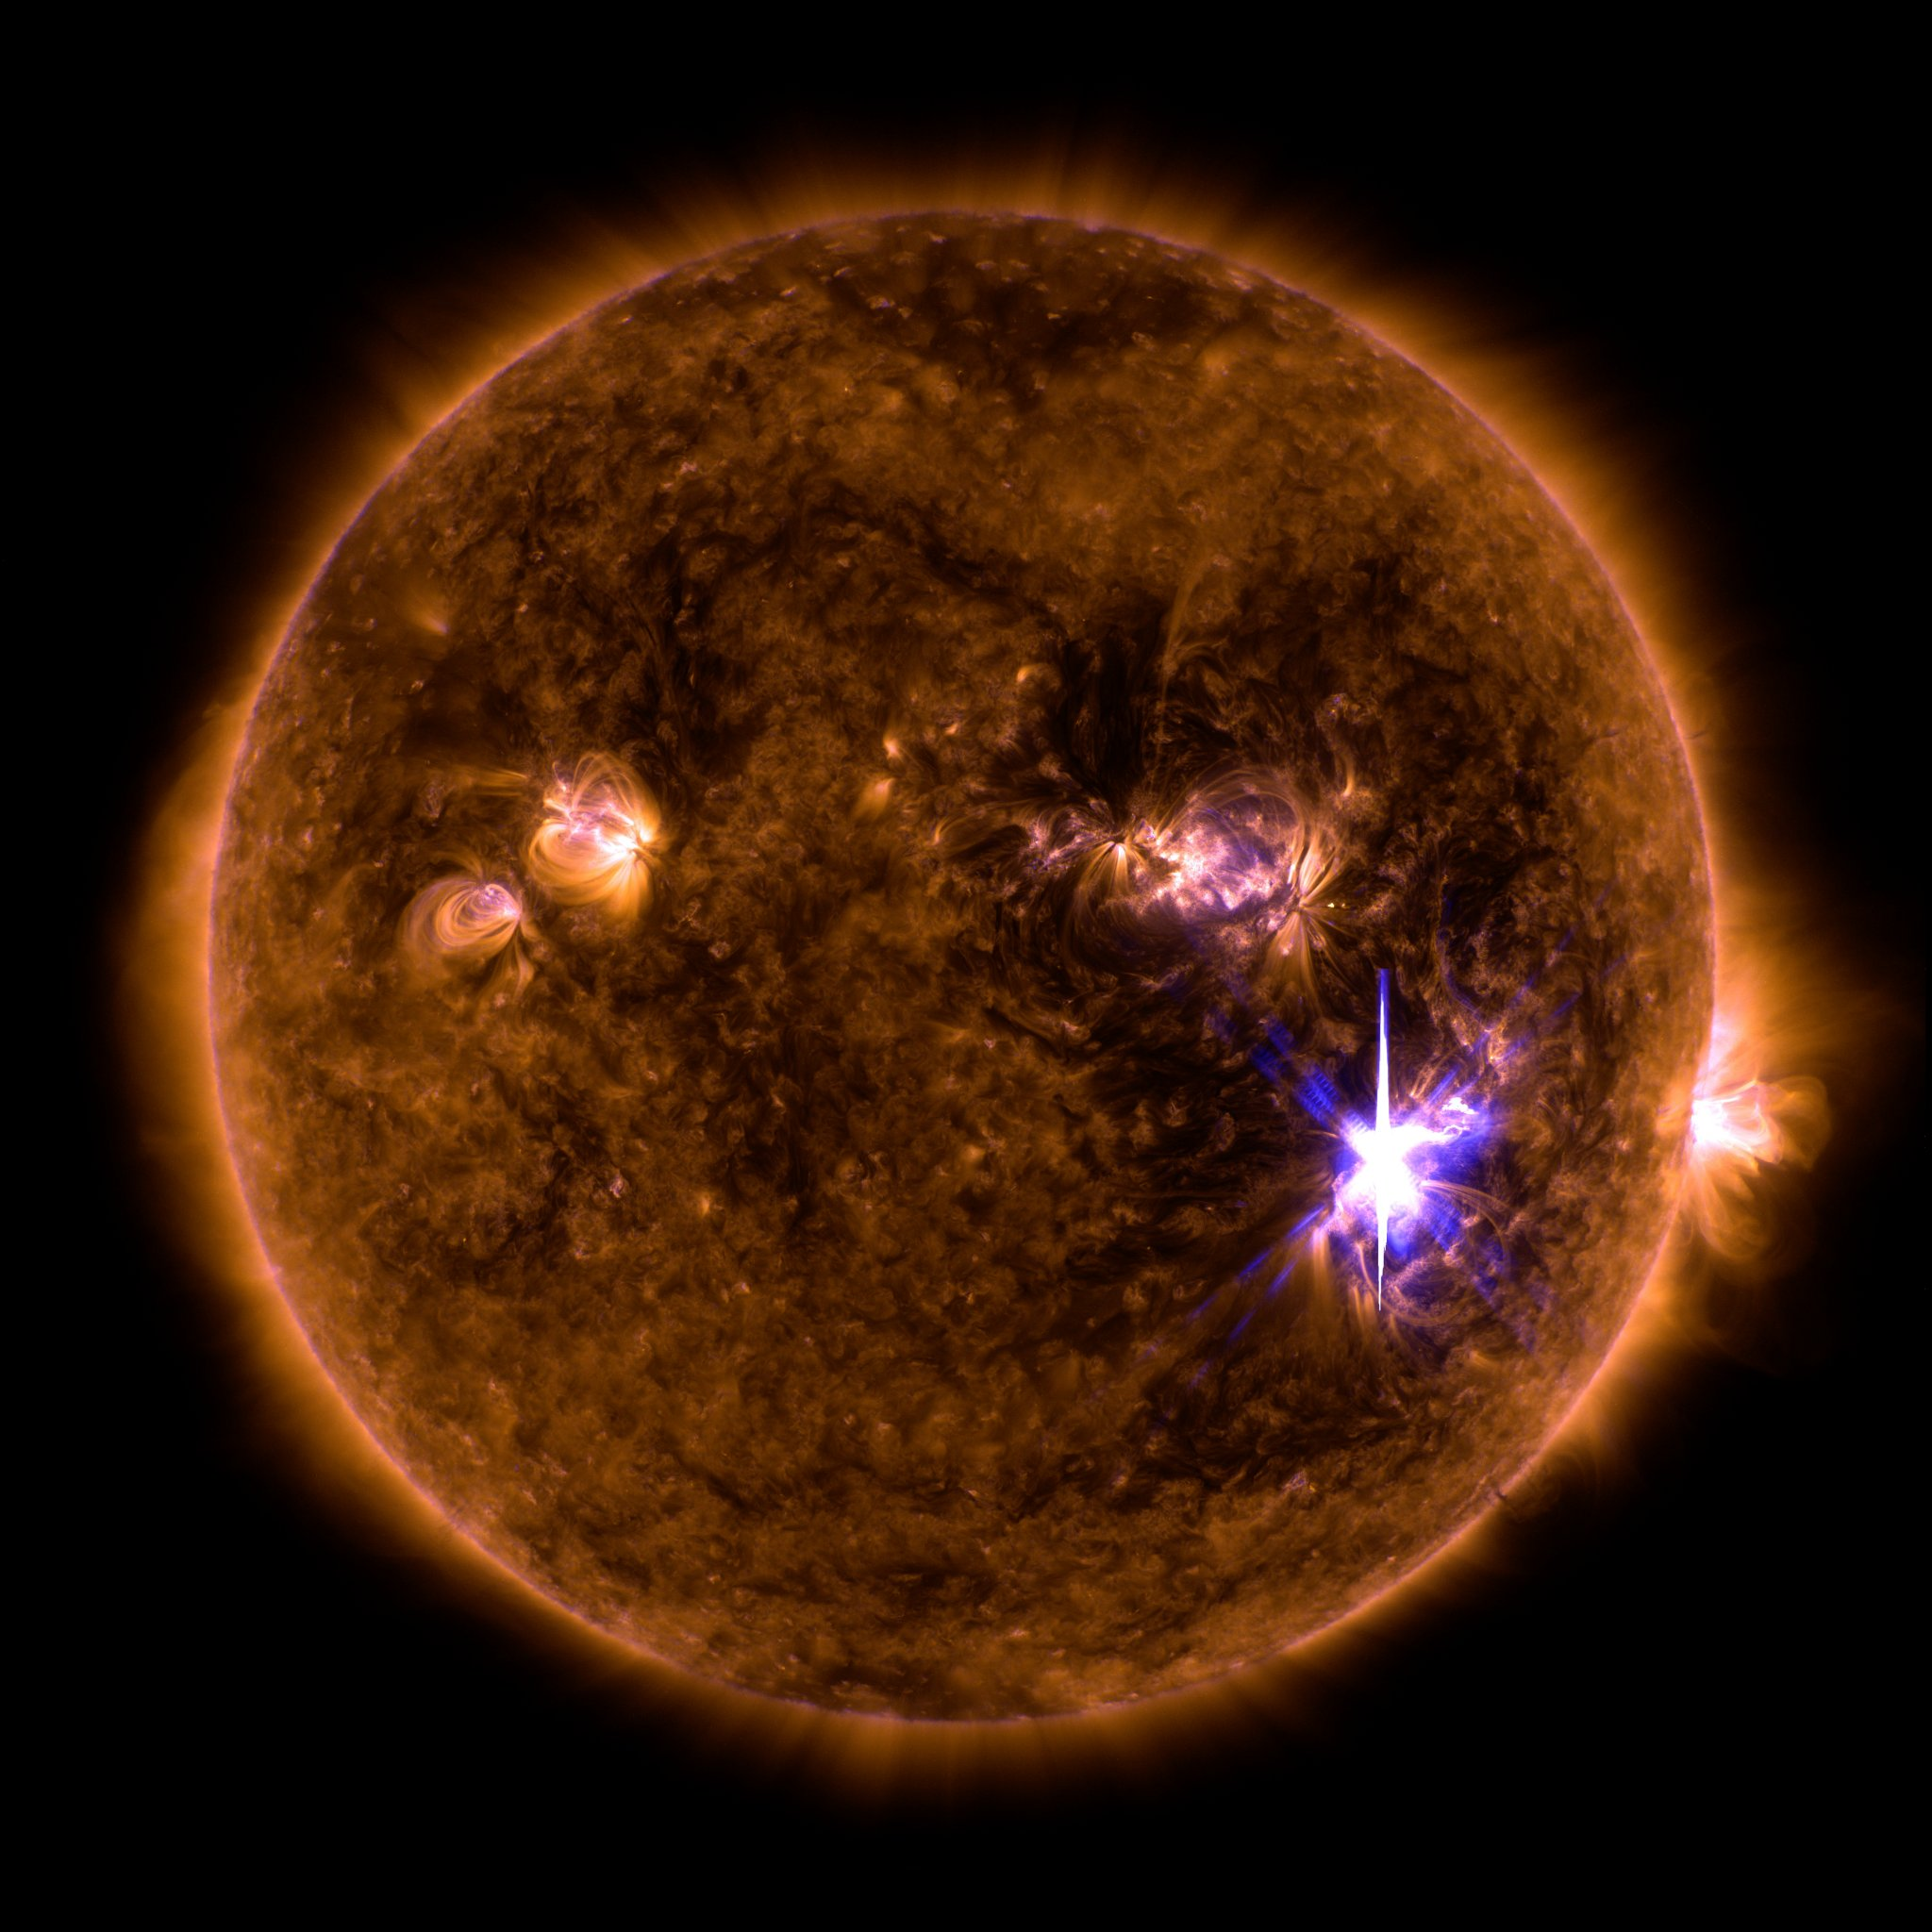
\includegraphics[width=3cm]{0906-sun.jpg}
\caption{6日に発生した太陽フレア}
\end{figure}

\section*{速報:9/7の太陽フレアについて}
9/7 14:41(UTC)に,またXクラスの太陽フレアが発生しました.
